
\chapter{Connessione degli host domotici alla VPN}
\label{ch:connessione-host-domotici}

\section{Overview della configurazione}

L'ultima parte della configurazione consiste nel rendere disponibile nella VPN la rete locale del \textit{router 4g}, consentendo quindi lo scambio di dati tra gli \textit{host-domotici} e i client della VPN.

Per simulare gli un host domotico è stata usata una \textit{raspberry pi}.

\begin{figure}[H]
    \centering
    \savebox{\myimage}{
        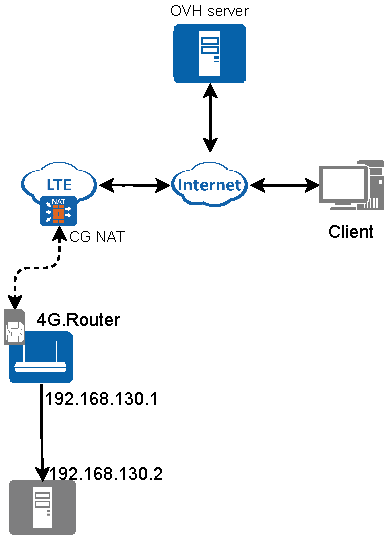
\includegraphics[width=0.44\linewidth]{immagini/diag2-host_real}
    }
    \begin{subfigure}{0.44\linewidth}
        \centering
        \usebox{\myimage}
        \caption{Diagramma della configurazione iniziale}
        \label{fig:diag2-host}
    \end{subfigure}
    \hfill
    \begin{subfigure}{0.53\linewidth}
        \centering
        \raisebox{\dimexpr.5\ht\myimage-.6\height\relax}{
            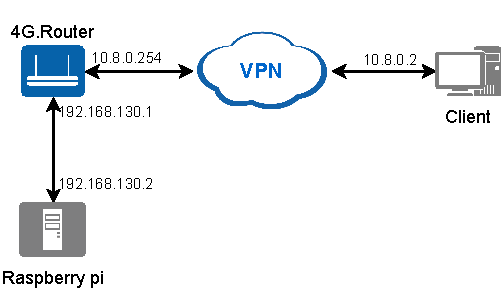
\includegraphics[width=1\linewidth]{immagini/diag2-host_virtual}
        }
        \caption{Diagramma finale}
        \label{fig:diag2-host1}
    \end{subfigure}
    \caption{Schemi concettuali della configurazione iniziale e finale per il capitolo \ref{ch:connessione-host-domotici}}
\end{figure}

\section{Creazione della firewall zone per la VPN} 

Per rendere possibile la comunicazione tra la rete \textit{lan} del \textit{Router} e la VPN è necessario configurare opportunamente il firewall.

Ciò viene fatto direttamente da LuCI, nella sezione firewall si avranno preconfigurate 2 zone, lan e wan, come si vede figura \ref{fig:luci-firewall-init}.

% TODO cambiare caption
\begin{figure}[H]
    \centering
    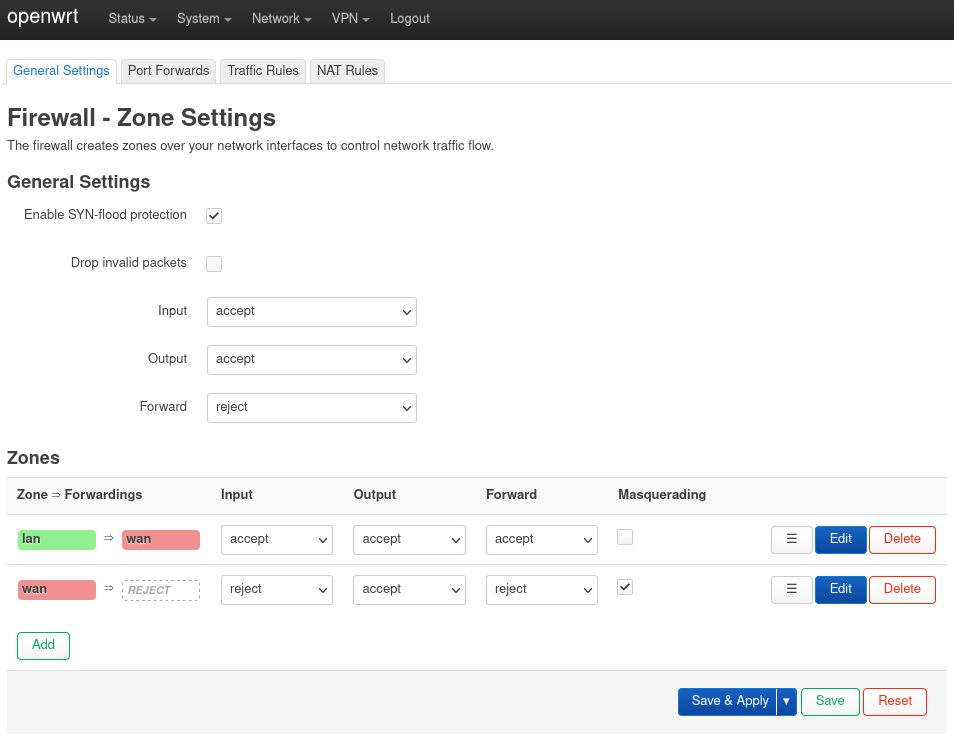
\includegraphics[width=0.9\linewidth]{immagini/LuCI_firewall_init1}
    \caption{Configurazione iniziale del firewall}
    \label{fig:luci-firewall-init}
\end{figure}

Si deve quindi aggiungere una nuova zona, chiamata vpn, con le seguenti opzioni:
\begin{itemize}
    \item Policy di forward: accept
    \item Forward consentito verso la zona lan
    \item Forward consentito dalla zona lan
\end{itemize}

Possiamo vedere la pagina di configurazione:

% TODO forse è meglio se le 2 figure stanno vicine


\begin{figure}[H]
    \centering
    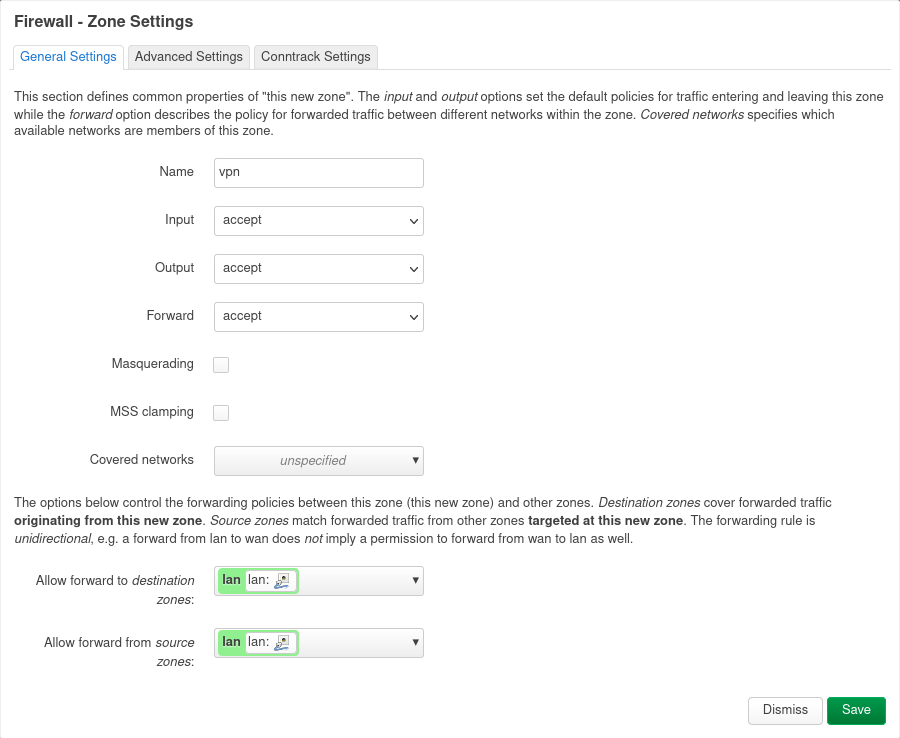
\includegraphics[width=0.9\linewidth]{immagini/LuCI_firewall_vpn1}
    \caption{Configurazione del firewall}
    \label{fig:luci-firewall-vpn}
\end{figure}

Dopo aver salvato, la pagina del firewall sarà:

% TODO cambiare caption
\begin{figure}[H]
    \centering
    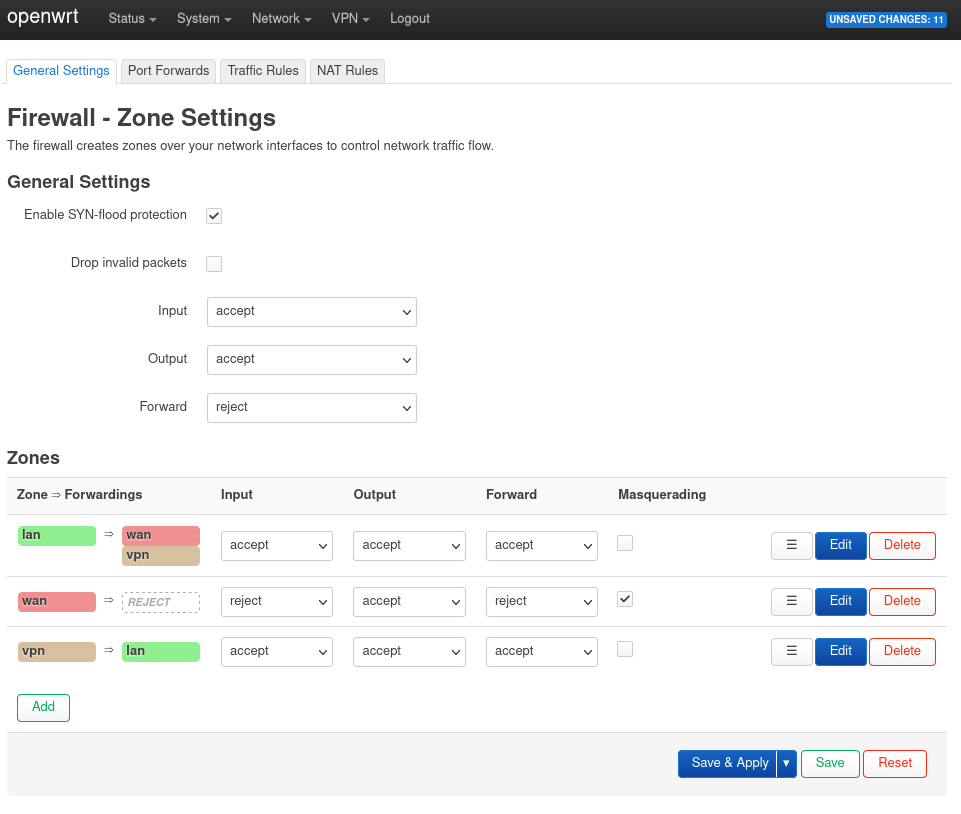
\includegraphics[width=0.9\linewidth]{immagini/LuCI_firewall_end1}
    \caption{Configurazione finale del firewall}
    \label{fig:luci-firewall-end}
\end{figure}

\section{Aggiunta dell'interfaccia tun0 alla zona vpn}

Per rendere attiva la zona firewall appena creata gli si deve assegnare almeno un'interfaccia, in questo caso gli si deve assegnare l'interfaccia tun0.

Ciò va fatto da LuCI, nella sezione \textit{interfaces}. Si deve quindi aggiungere una nuova interfaccia con le seguenti opzioni:
\begin{itemize}
    \item Name: tun0
    \item Proto: static
    \item Device: tun0
    \item ipv4 address: 10.8.0.254
    \item ipv4 netmask: 255.255.255.0
    \item Assign firewall zone: vpn
\end{itemize}

\begin{figure}[H]
    \centering
    \begin{subfigure}{0.9\linewidth}
        \centering
        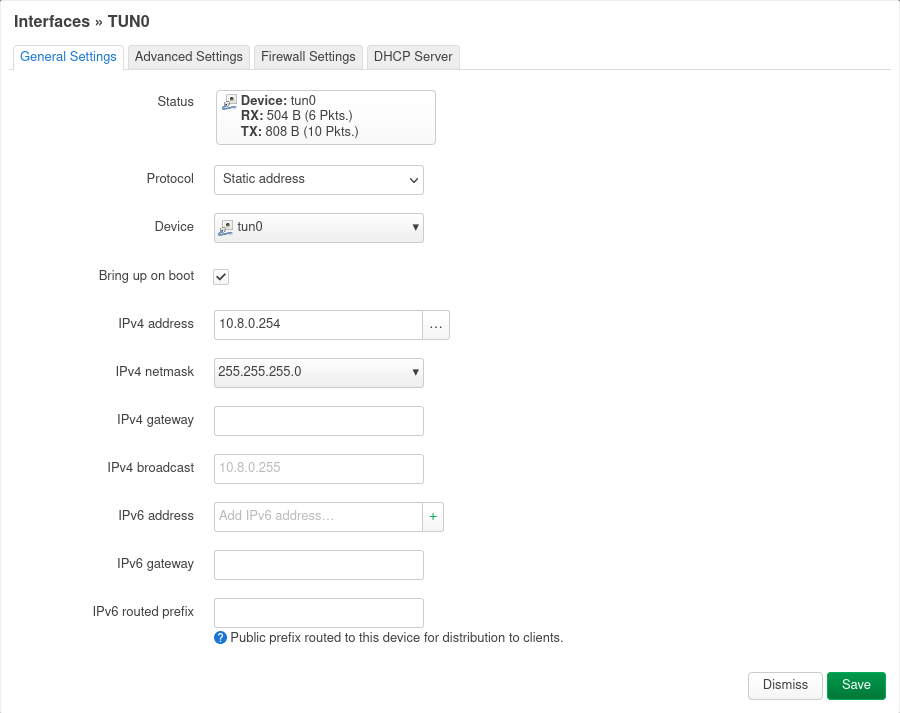
\includegraphics[width=0.9\linewidth]{immagini/LuCI_int_tun0_1}
        \caption{General settings}
        \label{fig:luci-firewall-interfaces}
    \end{subfigure}
    \medskip

    \begin{subfigure}{0.9\linewidth}
        \centering
        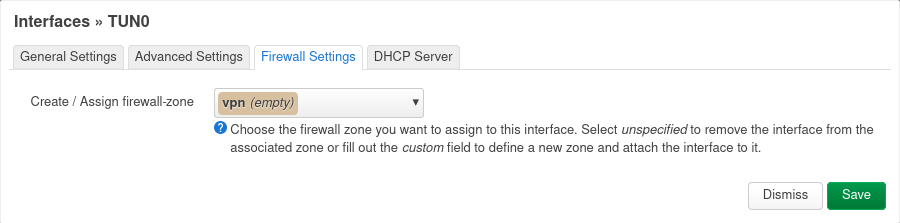
\includegraphics[width=0.9\linewidth]{immagini/LuCI_int_tun0_2}
        \caption{Firewall settings}
        \label{fig:luci-firewall-interfaces1}
    \end{subfigure}
    \caption{Assegnazione interfaccia \textit{tun0} alla zona firewall \textit{vpn} tramite interfaccia LuCI}
\end{figure}


\section{Modifiche alla configurazione OpenVPN del server}

Per instaurare una comunicazione bidirezionale tra \textit{host-domotico} e \textit{client} è necessario che:

\begin{enumerate}
    \item il server vpn sia consapevole che il \textit{router} vuole esporre una sua sottorete verso la vpn
    \item il client abbia l'opportuna rotta per raggiungere la sottorete dove si trova l'\textit{host-domotico}
\end{enumerate}

Per il punto 1 è necessario aggiungere la seguente riga nel file \\\code{/etc/openvpn/server/ccd/router}:

\begin{bashcode}{Server}{}
$ vim /etc/openvpn/server/ccd/router
ifconfig-push 10.8.0.254 255.255.255.0
iroute 192.168.130.0 255.255.255.0
$ vim /etc/openvpn/server/server.conf
169 route 192.168.130.0 255.255.255.0  # aggiungo la rotta nel server
\end{bashcode}

Per il punto 2 è necessario aggiungere la seguente riga alla configurazione OpenVPN nel \textit{Server}:

\begin{bashcode}{Server}{}
$ vim /etc/openvpn/server/server.conf
168 push "route 192.168.130.0 255.255.255.0"
\end{bashcode}

Dopo aver modificato la configurazione del server va riavviarlo con \code{systemctl restart}.

% TODO da rivedere
In questo modo nella procedura di connessione alla VPN, i client aggiungeranno la rotta verso la sottorete \code{192.168.130.0/24} nella loro tabella di routing. Possiamo verificarlo con: 

\begin{bashcode}{Client}{}
$ ip route
[...]
192.168.130.0/24 via 10.8.0.1 dev tun0
\end{bashcode}

\section{Test della configurazione}
\todo[da scrivere di più per i test, sono importanti, forse mettere qualcosa sul troubble shooting... mhhh]


Per testare la connessione tra \textit{client} e \textit{host-domotico} usiamo sia \code{ping} che \code{tracepath}, possiamo inoltre usare \code{tcpdump} sul \textit{Server} e \textit{Router} per vedere il percorso dei pacchetti.

Vediamo quindi un ping dal client verso l'\textit{host-domotico}, con server e router in ascolto sull'interfaccia tun0:

\begin{bashcode}{Client}{}
$ ping -c 1 192.168.130.3
PING 192.168.130.3 (192.168.130.3) 56(84) bytes of data.
64 bytes from 192.168.130.3: icmp_seq=1 ttl=63 time=0.643 ms

--- 192.168.130.3 ping statistics ---
1 packets transmitted, 1 received, 0% packet loss, time 0ms
rtt min/avg/max/mdev = 0.643/0.643/0.643/0.000 ms
\end{bashcode}


\begin{bashcode}{Server}{}
$ tcpdump -i tun0
listening on tun0, link-type RAW (Raw IP), snapshot length 262144 bytes
\end{bashcode}

Il server non ha visto traffico poiché ha l'opzione \code{client-to-client} abilitata, ciò comporta che il layer vpn effettua il routing senza passare per l'interfaccia di rete del router.

\begin{bashcode}{Router}{}
$ tcpdump -i tun0
listening on tun0, link-type RAW (Raw IP), capture size 262144 bytes
10:44:07.228387 IP 10.8.0.2 > host-domotico: ICMP echo request, id 12, seq 1, length 64
10:44:07.228550 IP host-domotico > 10.8.0.2: ICMP echo reply, id 12, seq 1, length 64
\end{bashcode}

Il router vede il pacchetto e lo instrada verso l'host corretto.

Provando nella direzione inversa si ottiene lo stesso risultato

\begin{bashcode}{Host-domotico}{}
$ ping -c 1 10.8.0.2
PING 10.8.0.2 (10.8.0.2) 56(84) bytes of data.
64 bytes from 10.8.0.2: icmp_seq=1 ttl=63 time=0.428 ms

--- 10.8.0.2 ping statistics ---
1 packets transmitted, 1 received, 0% packet loss, time 0ms
rtt min/avg/max/mdev = 0.428/0.428/0.428/0.000 ms
\end{bashcode}

e il router vede:

\begin{bashcode}{Router}{}
$ tcpdump -i tun0
listening on tun0, link-type RAW (Raw IP), capture size 262144 bytes
11:56:10.469901 IP host-domotico > 10.8.0.2: ICMP echo request, id 14, seq 1, length 64
11:56:10.470230 IP 10.8.0.2 > host-domotico: ICMP echo reply, id 14, seq 1, length 64
\end{bashcode}

% TODO da espandere
Possiamo inoltre usare \code{tracepath} per vedere gli hop:

\begin{bashcode}{Client}{}
$ tracepath 192.168.130.3
1?: [LOCALHOST]                      pmtu 1500
1:  10.8.0.254                       0.471ms
1:  10.8.0.254                       0.473ms
2:  192.168.130.3                    0.567ms reached
    Resume: pmtu 1500 hops 2 back 2
\end{bashcode}

\begin{bashcode}{host-domotico}{}
$ tracepath 10.8.0.2
1?: [LOCALHOST]                      pmtu 1500
1:  router-1                         0.062ms
1:  router-1                         0.068ms
2:  10.8.0.2                         0.592ms reached
    Resume: pmtu 1500 hops 2 back 2
\end{bashcode}

